\chapter{Range-Rename}
\label{chap:rename}

This chapter describes the \bet operation, range-rename, that makes efficient
renames possible on full-path-indexed \betrfs.
To perform a rename, \betrfs simply calls the range-rename function of \fti,
which updates all related key/value pairs in the underlying \bets efficiently.
This chapter starts by describing the range-rename interface,
followed by two key techniques that make efficient range-rename operation
possible on \bets, \textbf{tree surgery} and \textbf{key lifting}.
At last, this chapter discusses the changes that \betrfs makes to adopt
range-renames.

\section{The range-rename interface}

Range-rename is a new key/value store function defined as:
range-rename(\spre, \dpre).
Define a source key/value pair as a key/value pair whose key has prefix \spre
and a destination key/value pair as a key/value pair whose key has prefix \dpre.
Range-rename(\spre, \dpre) does three things:
\begin{itemize}
\item it deletes all destination key/value pairs from the key/value store;
\item then, for any source key/value pair $(k,v)$ in the key/value store,
it inserts a key/value pair $(k',v)$ to the key/value store,
where $k$ is the concatenation of \spre and some suffix $s$ and $k'$ is the
concatenation of \dpre and the same suffix $s$;
\item at last, it deletes all source key/value pairs from the key/value store.
\end{itemize}
In other words, a range-rename deletes all destination key/value pairs and
updates all source key/value pairs to have \dpre.

To see how range-rename accomplishes renames in full-path-indexed \betrfs,
consider renaming file ``/foo'' to ``/bar''.
In \mdb, \betrfs needs to insert the destination key ``/bar''
(this insert overwrites the old value of ``/bar'', if it exists)
and delete the source key ``/foo'', resulting in two function calls to \fti.
On the other hand, in \ddb, \betrfs needs to delete all data keys of ``/bar''
(POSIX allows file renames to overwrite the destination file) and update all
data keys of ``/foo'' to be data keys of ``/bar''.
The whole work in \ddb can be done by calling range-rename(``/foo'',``/bar'')
(data keys are the concatenation of the full-path and an 8-byte block number).

Similarly, consider renaming directory ``/baz'' to ``/qux''.
In \mdb, \betrfs also needs to insert the destination key ``/qux'' and deletes
the source key ``/baz'' with two functions calls to \fti.
Additionally, \betrfs needs to update all keys with prefix ``/baz/'' to have
prefix ``/qux/''
(POSIX only allows directory renames to overwrite an empty directory, which
means there cannot be any key with prefix ``/qux/''),
which is covered in range-rename(``/baz/'', ``/qux/'').
Likewise, in \ddb, \betrfs also needs to update all keys with prefix ``/baz/''
to have prefix ``/qux/'', which is done in range-rename(``/baz/'', ``/qux/'')
(directory doesn't have any data key).

In summary, full-path-indexed \betrfs can finish a file rename by calling three
functions of \fti: an insert, a delete and a range-rename.
And a directory rename can be done with an insert, a delete and two
range-renames.
Therefore, efficient renames are possible in full-path-index \betrfs if
\fti can perform range-renames efficiently on the underlying \bets.

\section{Range-rename on \bets}

This section describes the approach to do a range-renames on the \bet
with a bounded number of IOs.
The efficient range-rename requires lexicographic key order so that keys with
the same prefix are contiguous in the key space.
With contiguous keys, it is possible to have an isolated subtree that contains
and only contains all key/value pairs of a certain prefix.
The range-rename performs \textbf{tree surgery} to create such an isolated
subtree.
Then, the range-rename moves the subtree to another location on the \bet and
updates the prefixes of keys in the subtree through \textbf{key lifting}.

This section first describes tree surgery and key lifting, and then shows how
range-rename can be done with these two techniques.

\subsection{Tree surgery}

\begin{figure}
    \begin{subfigure}{\textwidth}
        \centering
        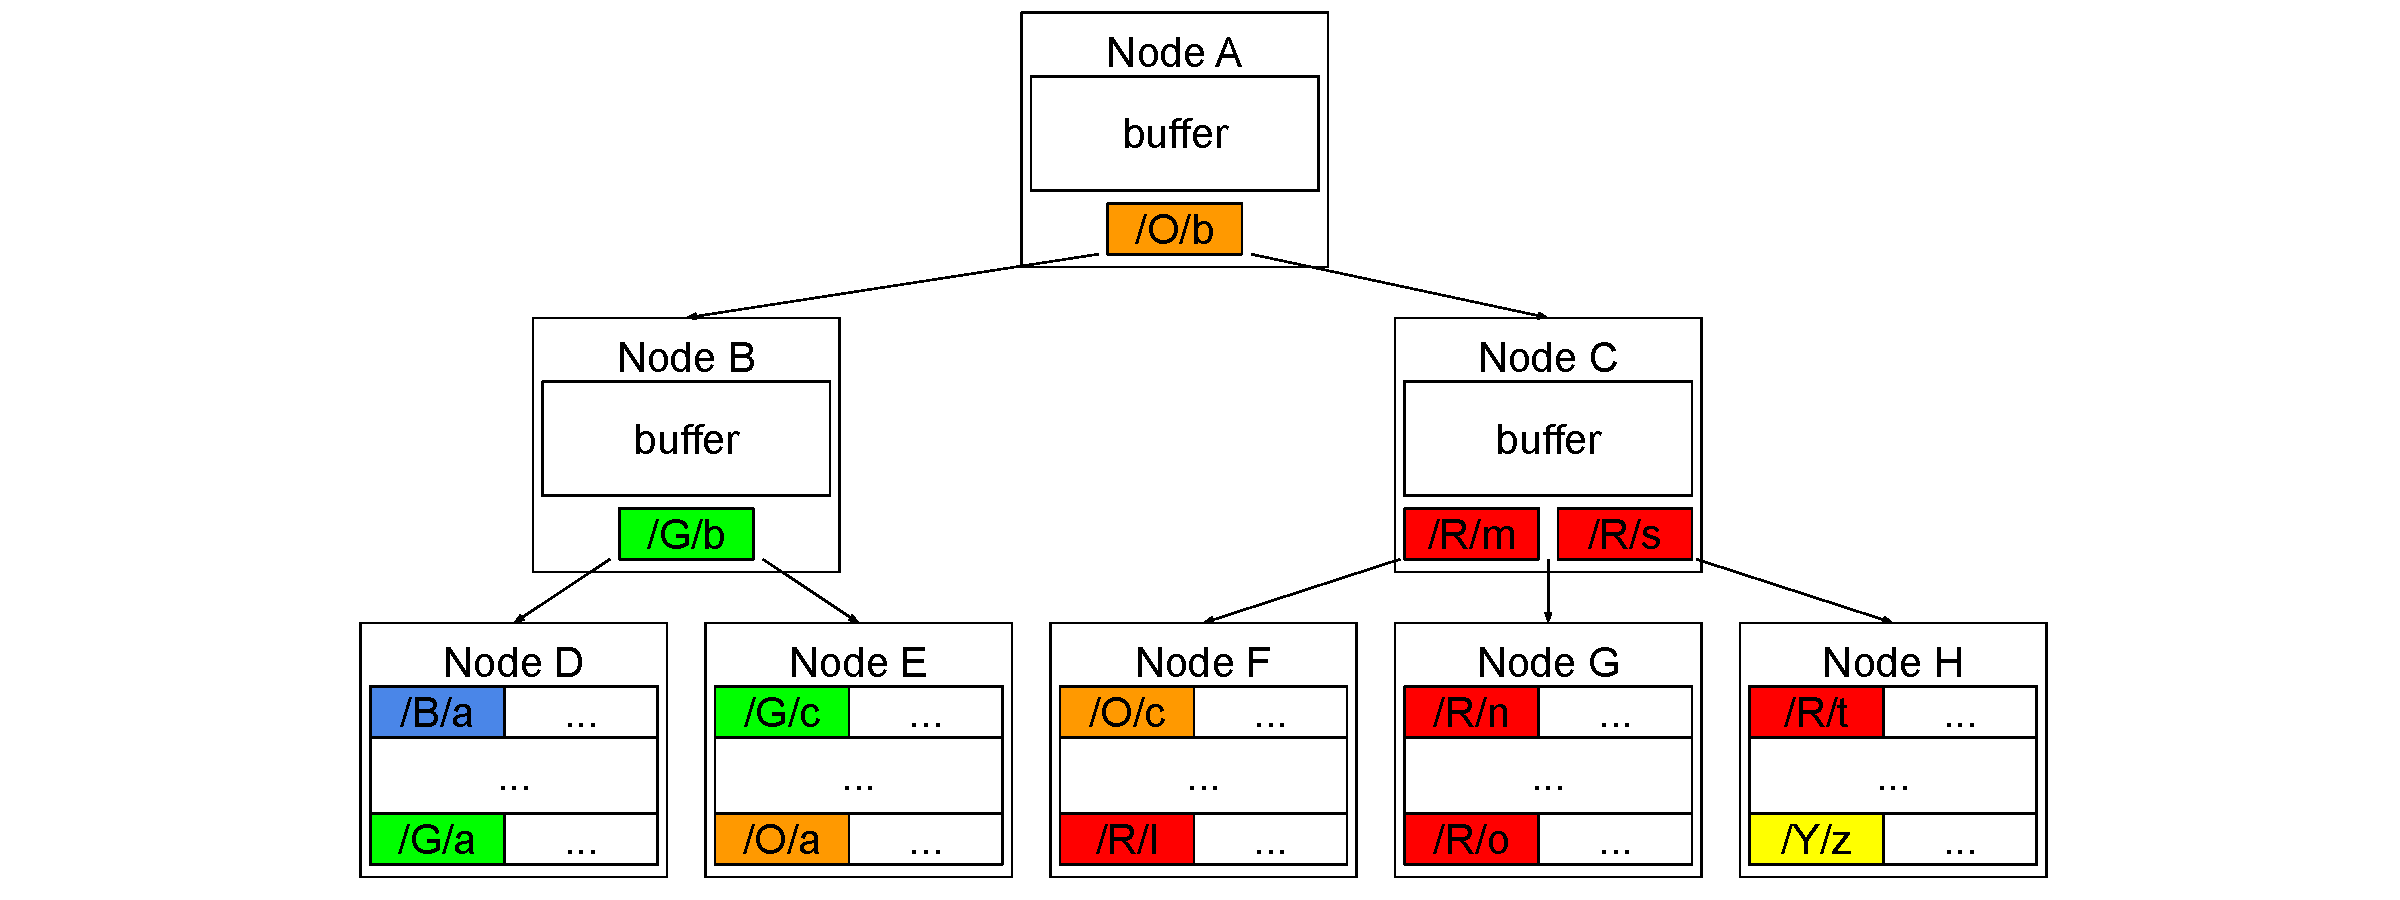
\includegraphics[width=.9\linewidth]{fig/slice-1}
        \caption{\label{subfig:slice-1} The \bet before tree surgery.}
    \end{subfigure}
    \begin{subfigure}{\textwidth}
        \centering
        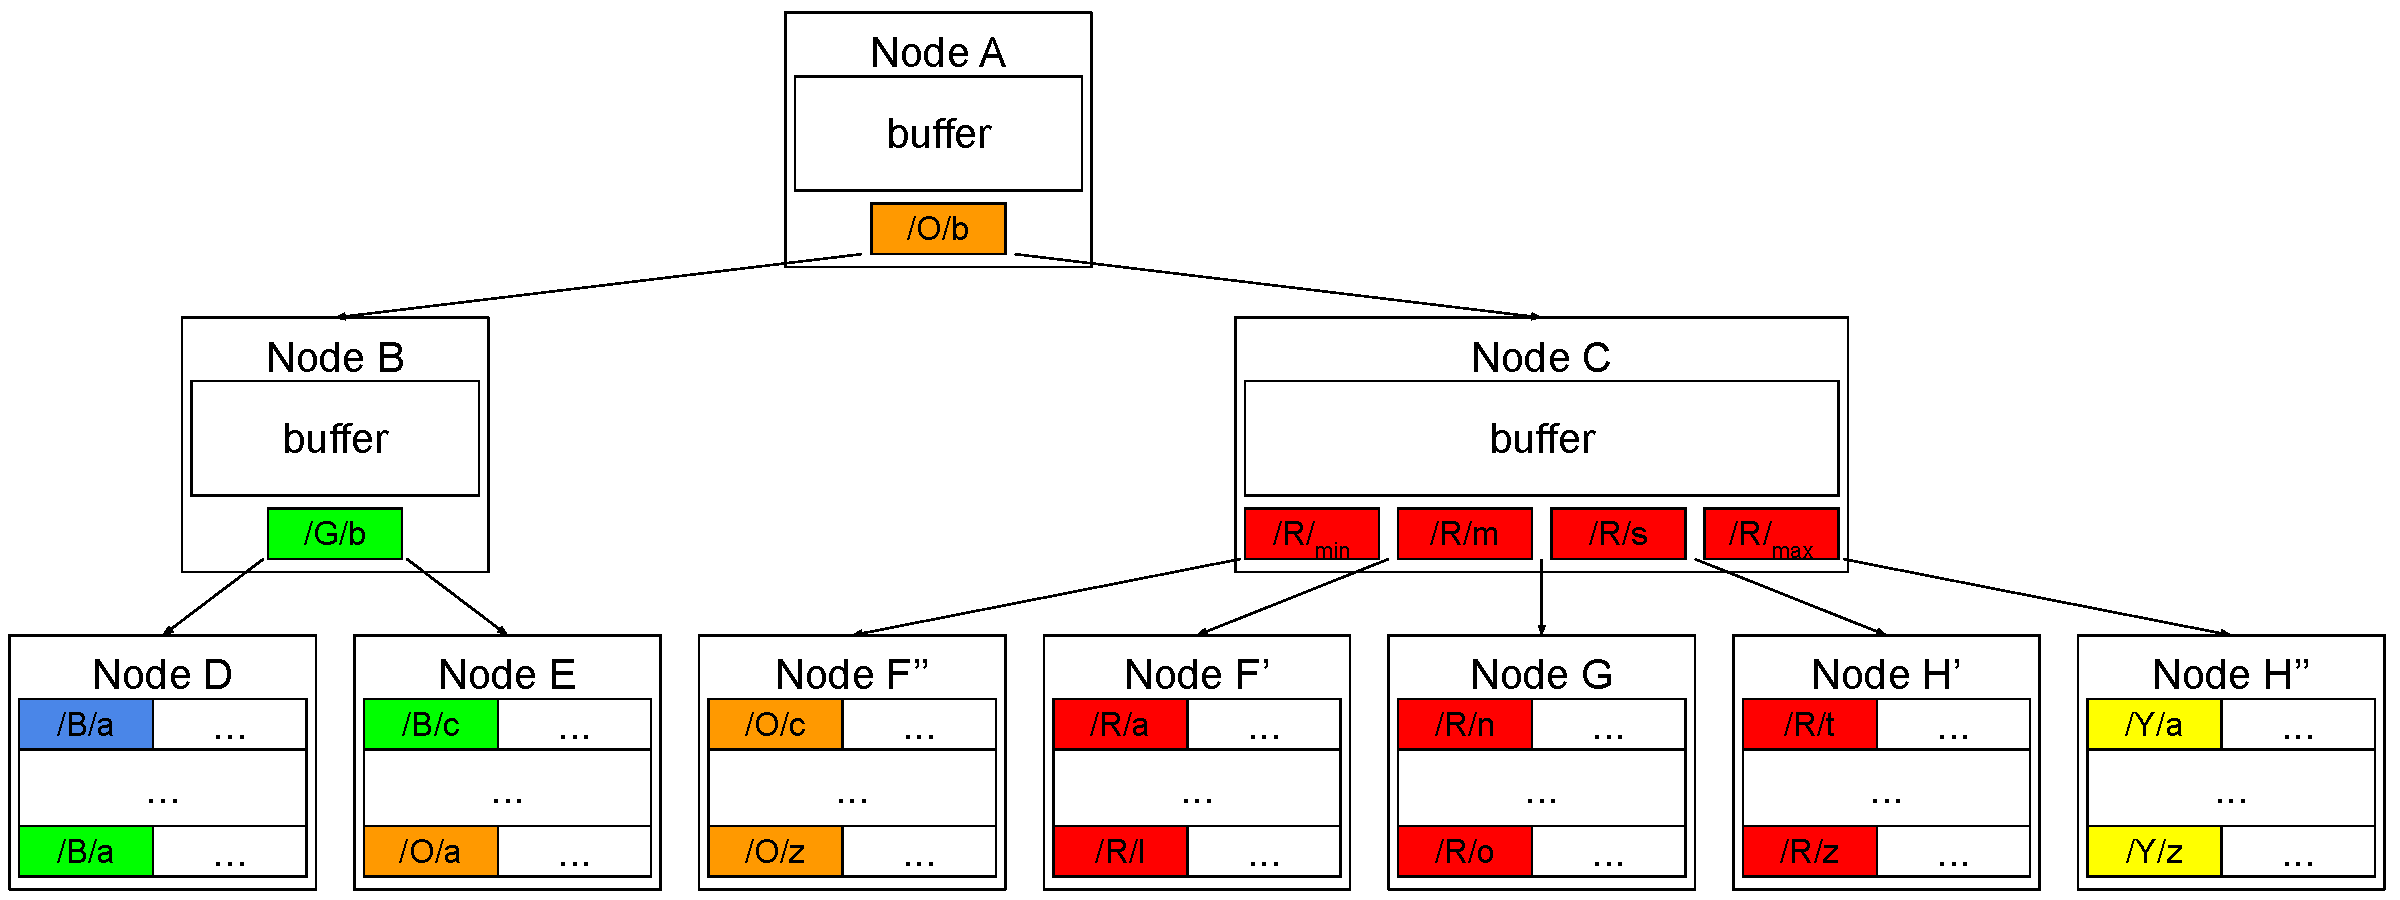
\includegraphics[width=.9\linewidth]{fig/slice-2}
        \caption{\label{subfig:slice-2} Tree surgery splits leaf nodes.}
    \end{subfigure}
    \begin{subfigure}{\textwidth}
        \centering
        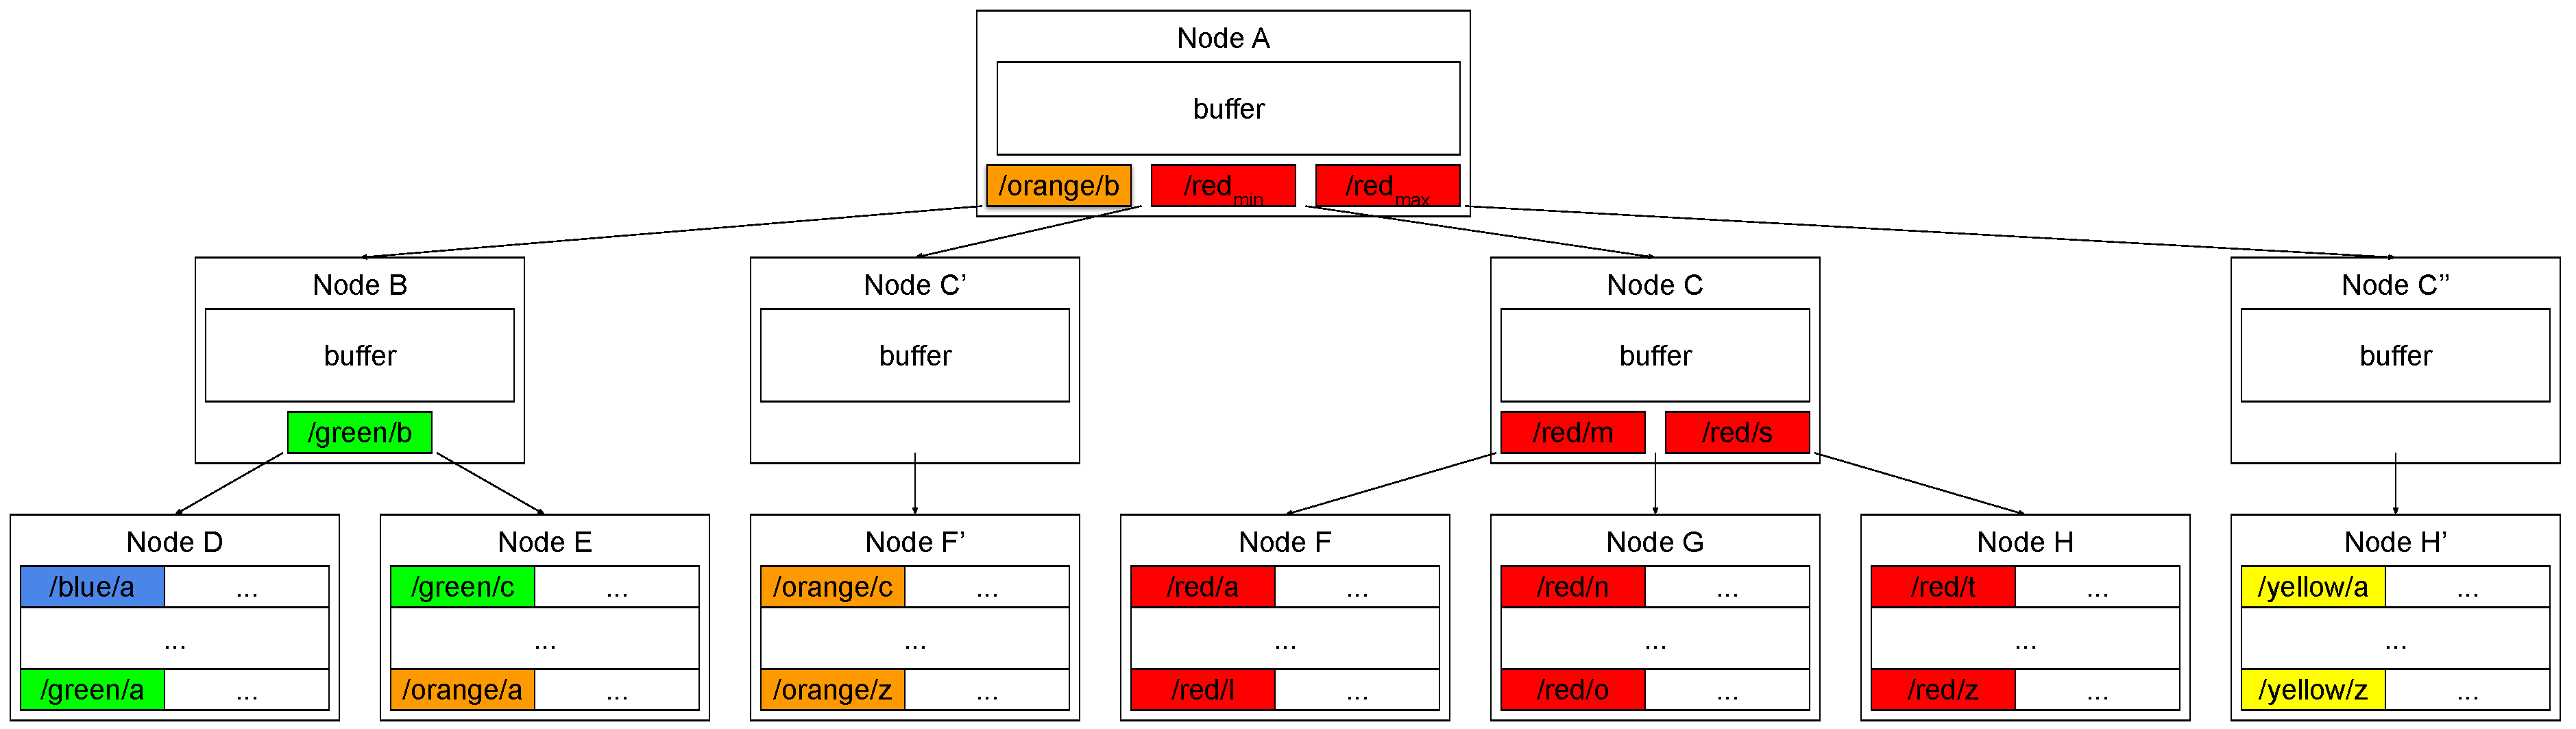
\includegraphics[width=.9\linewidth]{fig/slice-3}
        \caption{\label{subfig:slice-3} Tree surgery splits the LCA.}
    \end{subfigure}
    \caption[Tree surgery example]{\label{fig:slice}
        Tree surgery slices out an isolated subtree of prefix ``/red/''.}
\end{figure}

The goal of tree surgery is to create an isolated subtree of a certain
prefix $p$ on the \bet.
In the \bet, each node covers a certain key range, bounded by the key range and
pivots of its parent.
For a certain key range $(p_{min}, p_{max})$ ($p_{min}$ and $p_{max}$ are the
minimum and maximum keys with prefix $p$, respectively), there are three types
of nodes: nodes whose range are completely out of the key range, nodes whose
range are completely in the key range, and nodes whose range partly overlapped
with the key range (called \textbf{fringe nodes}).

Figure~\ref{subfig:slice-1} shows an example of a \bet.
Node A, B and C are non-leaf nodes with buffers and pivots.
Node D, E, F, G and H are leaf nodes that only store key/value pairs.
Parent-to-leaf pointers in the figure link all nodes into a tree.
Consider prefix ``/red/'',
Node B, D and E are completely out of the key range $(/red/_{min}, /red/_{max})$,
Node G is completely in the key range, and other nodes are fringe nodes.

\paragraph{Identifying fringe nodes.}
The first step of tree surgery is to identify all fringe nodes.
This is done by performing root-to-leaf traversals with two keys,
$p_{min}$ and $p_{max}$.
because a fringe node must have one of the two keys in its range.

An important fringe node for tree surgery is the \textbf{LCA}
(Lowest Common Ancestor) of two keys: the LCA is the \bet node lowest in the
tree on the search path for both keys (and hence including all keys in between).
In Figure~\ref{subfig:slice-1}, Node C is the LCA.
The subtree rooted at the LCA is the lowest subtree in the \bet that covers
the whole range $(p_{min}, p_{max})$.
And tree surgery uses this subtree to create its isolated subtree by splitting
nodes.
While traversing the \bet, tree also flushes messages in the fringe node from
parent to child to ensure that no message stays above the subtree.

\paragraph{Slicing.}
The second step is to slice out the isolated subtree by splitting fringe nodes
from bottom up.
The goal of slicing to separated unrelated key/value pairs in the fringe nodes
from key/values in the range.
Slicing uses the same code used for standard \bet node splits, but slicing
divides the node at the slicing key, which is $p_{min}$ or $p_{max}$ rather than
picking a key in the middle of the node.

In Figure~\ref{subfig:slice-2}, tree surgery splits Node F with key
$/red/_{min}$, generating new Node F that only contains keys with prefix
``/red/'' and another Node F$'$ that doesn't contain another key with prefix
``/red/''.
Likewise, tree surgery splits Node H into new Node H and Node H$'$ with key
$/red/_{max}$.
At last, in Figure~\ref{subfig:slice-3}, tree surgery splits the LCA, Node C,
into new Node C, Node C$'$ and Node C$''$ with both keys, $/red/_{min}$ and
$/red/_{max}$.
The subtree rooted at the new Node C is the isolated subtree that contains and
only contains all keys with prefix ``/red/''.

\subsection{Key lifting}

\begin{figure}
    \begin{subfigure}{\textwidth}
        \centering
        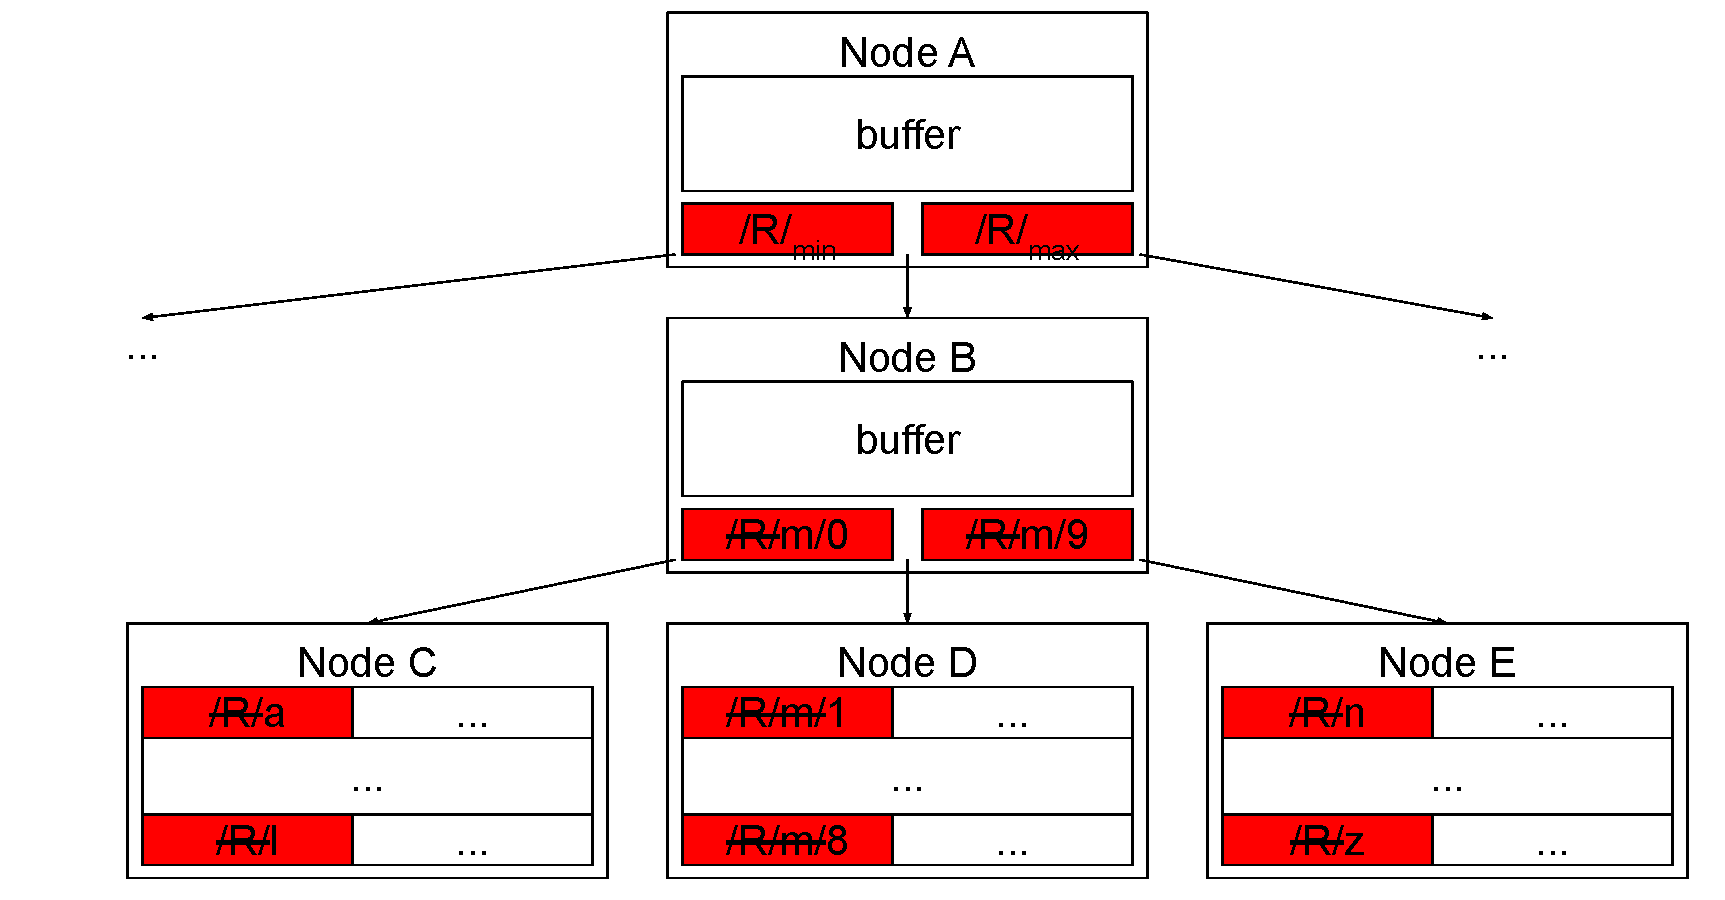
\includegraphics[width=.9\linewidth]{fig/lift-1}
        \caption{\label{subfig:lift-1} A subtree of ``/red/'' keys bounded by
            pivots $/red/_{min}$ and $/red/_{max}$ in the parent}
    \end{subfigure}
    \begin{subfigure}{\textwidth}
        \centering
        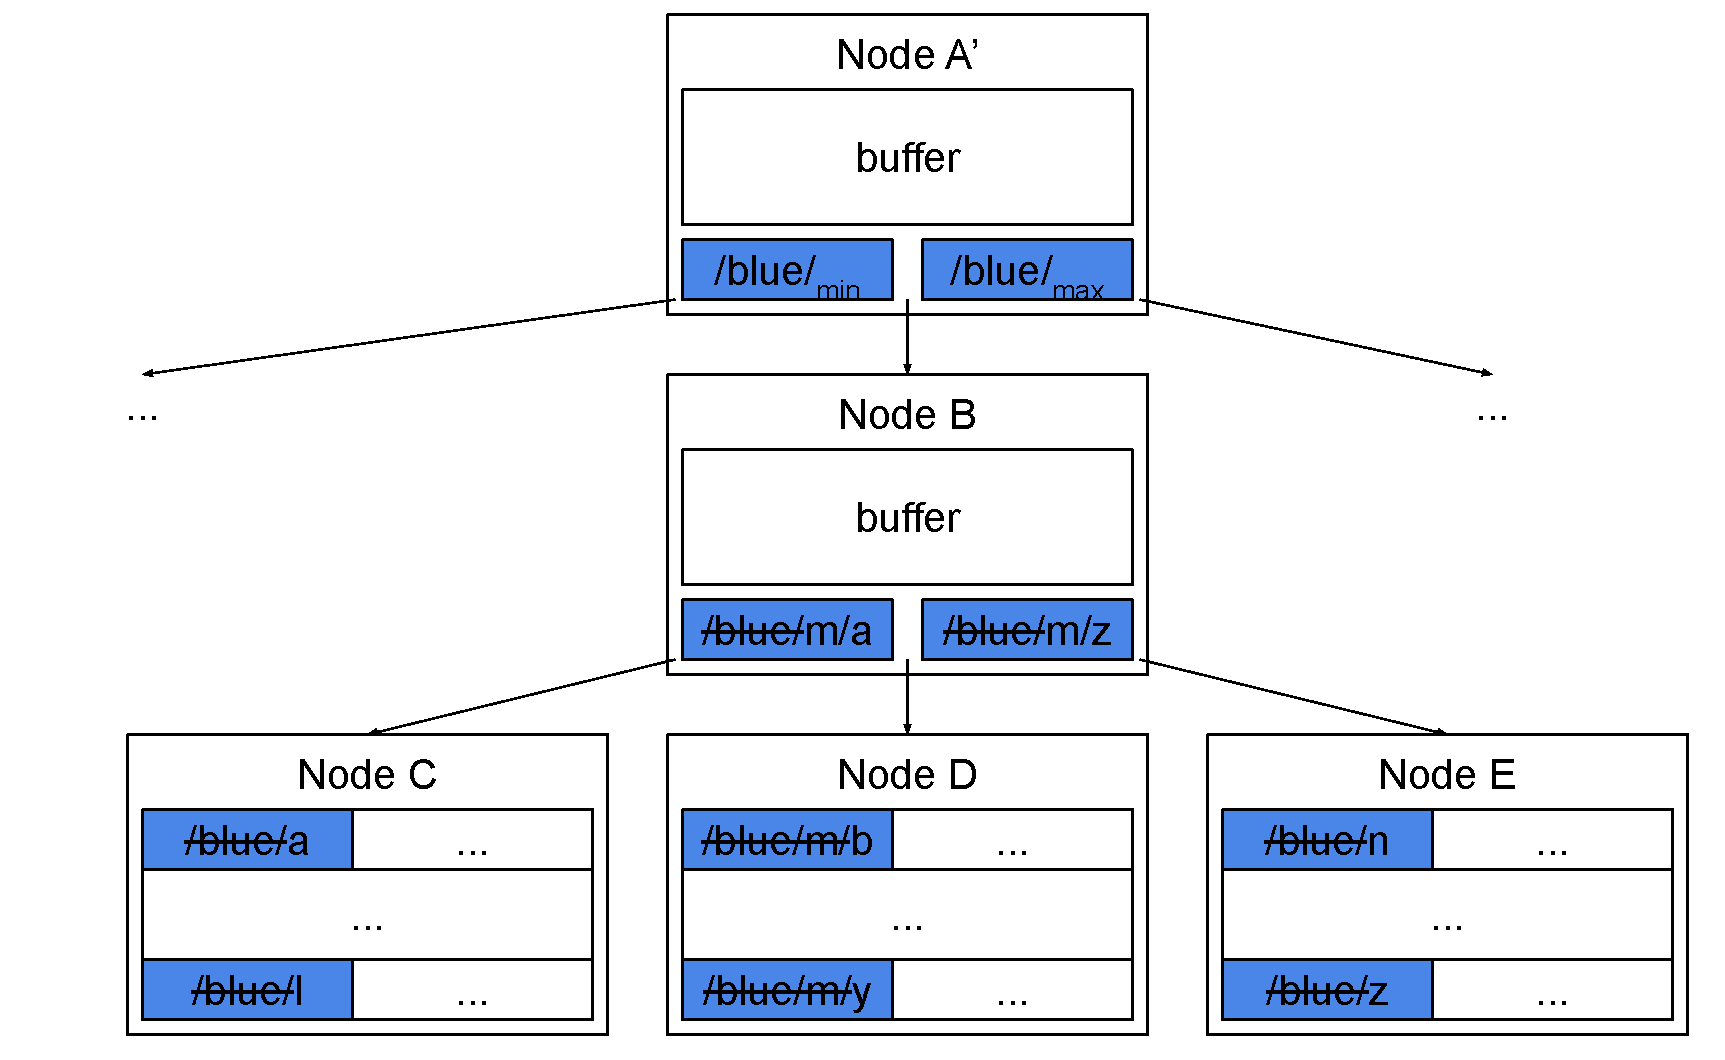
\includegraphics[width=.9\linewidth]{fig/lift-2}
        \caption{\label{subfig:slice-2} The same subtree bounded by pivots
            $/blue/_{min}$ and $/blue/_{max}$ in the parent}
    \end{subfigure}
    \caption[Key lifting example]{\label{fig:lift}
        Key lifting lifts prefixes from the subtree. Keys in the same subtree
        are viewed with different prefixes when the pivots in its parent
        changes.}
\end{figure}

Tree surgery slices out a subtree of a certain prefix, which can be moved to
another location in the \bet.
However, the keys in the subtree will not be coherent with the new location in
the tree.
As part of a range-rename, the prefixes of all keys in this subtree need to be
updated.
The particularly concerning case is when the subtree is a very large.
Updating the prefixes by traversing the subtree costs a lot of IOs, touching
nodes that would otherwise be untouched by the tree surgery.

Key lifting eliminates the need to update prefixes in the subtree by
transferring \bets to lifted \bets.
The idea of key lifting comes from the observation that with the lexicographic
order, all keys in the range of two pivots must have the same prefix that is
the \textbf{LCP} (Longest Common Prefix) of the pivots.
Therefore, this LCP is redundant information in the subtree of the two pivots
and can be removed from the subtree.

At a high level, each parent in a lifted \bet stores each child's common,
lifted key prefix alongside the pointer to the child.
Child nodes only store differing key suffixes.
This approach encodes the complete key in the path taken to reach a given node
and one can then modify the prefix for a lifted subtree by only modifying the
parent node, eliminating the need to change key and pivot prefixes in all nodes
of a subtree.

For example, in Figure~\ref{subfig:lift-1}, the subtree rooted at Node B is
bounded by ``/red/$_{min}$'' and ``/red/$_{max}$'' in Node A.
Therefore, all keys in the subtree must have prefix ``/red/'' and key lifting
removes this prefix from the subtree (marked as strike-through in keys).
Likewise, Node D is bounded by ``m/a'' and ``m/z'' in Node B
(note ``/red/'' is already lifted from the sutbree rooted at Node B),
so key lifting removes the prefix ``m/'' from Node D.
In Figure~\ref{subfig:lift-2}, the same subtree, which contains exactly the
same key/value pairs, is moved to a different location, bounded by
``/blue/$_{min}$'' and ``/blue/$_{max}$'' in Node A.
Because the prefix encoded in the parent-to-child pointer in Node A' becomes
``/blue/'', all keys in the subtree have ``/blue/'' prefixes instead.

Key lifting doesn't introduce additional IOs to reads and writes on lifted
\bets.
Queries need to reconstruct the full key by concatenating prefixes during a
root-to-leaf traversal.
When flushing, the lifted prefix must be removed from messages being flushed
to the child.
A node split adds a pivot to the parent, changing the lifted prefix in the
parent-to-child pointer, so it needs to update keys in the resulting children.
However, this doesn't incur additional IO.
Similarly, no additional IO is required in node merges.

Key lifting is completely transparent to the application using the key/value
store.
From the file system's perspective, it is still storing key/value pairs with
full-path keys.

\subsection{Put them together}

\textbf{Figures Here}


\paragraph{Healing}  Our \bet implementation maintains the
invariant that all internal nodes have between 4 and 16 children,
which bounds the height of the tree.  After the transplant completes,
however, there may be a number of in-memory \bet nodes at the fringe
around the source and destination that have fewer than 4 children.

We handle this situation by triggering a rebalancing within the tree.
Specifically, if a node has only one child, the slicing process will merge
it after completing the work of the rename.
After the transplant completes, there may be a number
of \bet nodes in memory at the fringe around the
source and destination that have fewer children than desired.
The healing process merges these smaller nodes back together,
using the same approach as a typical \bet merge.  At this point, it is also
possible that this could trigger a rebalancing within the tree.

One very important optimization we found as part of healing was to
agressively merge {\em stalks}, or new descendants of an LCA with
only a single child.
When the source and destination LCA are at different height, slicing
will creates some nodes with a single child.
Traversing these stalks undermines the logarithmic search time one would
expect from a tree, and created significant performance overheads.
After healing, we immediately merge nodes at the fringe
to a normal fanout in \bet.

\paragraph{Crash Consistency} \betrfs relies on three on-disk data structures to
ensure crash consistency: the trees, a block table indicating the disk blocks
used by the trees, and a write-ahead redo log. In general, \betrfs ensures crash
consistency by appending pending messages to the redo log and then applying
messages to the tree in a copy-on-write manner.
At periodic intervals (by default every 60 seconds), \betrfs ensures that there
is a consistent, sharp checkpoint of the tree on disk.
After a crash, \betrfs reads the last checkpointed tree and replays the redo log
after the checkpoint.
Range rename works within this framework.

A range rename is {\em logically applied} to the tree as soon as
(1) the range-rename message is added to the redo log and
(2) tree surgery locks the root of the tree.
The range rename is durable as soon as the redo log entry is written to disk.
If the system crashes after a range rename is logged, the recovery will see a
prefix of the message history that includes the range-rename message, and the
tree surgery will be redone in response to the range-rename message.
After both the tree surgery and the subsequent checkpoint of the tree complete,
there is no need to repeat the tree surgery after a crash.

We note that the current implementation does tree surgery immediately after the
message is placed in the redo log.
It is possible to batch range rename messages and apply them lazily,
but we leave this for future work.
As a result of this choice, however, there are fewer cases to reason about
in understanding crash consistency.

Tree surgery walks down the tree and locks the nodes along the path
hand-over-hand until either the source LCA or the destination LCA is reached.
Then, until tree surgery completes, all fringe nodes, the LCAs, and the parents
of LCAs are locked in memory and dirtied.
Upon tree surgery completion, these nodes will be unlocked.
Because the checkpoint process must grab the locks of all involved node before
writing them to disk,
no intermediate state of slicing will be exposed to a checkpoint.
Dirty nodes may be written back to disk, copy-on-write, before checkpointing
under memory pressure.
However, because the recovery process always starts from the last checkpoint and
the last block table in which these newly allocated nodes is not reachable,
these nodes with uncheckpointed state will be marked as free during crash
recovery.

If the system crashes after tree surgery begins but before surgery completes,
the recovery code will see a consistent checkpoint of the tree as it was
before the tree surgery.
The same is true if the system crashes after tree surgery but before dirty nodes
are written back to disk.
Because a checkpoint flushes all dirty nodes, if the system crashes after a
checkpoint, all nodes affected by tree surgery will be on disk.
We checked this functionality with crash recovery unit tests.
We ran the system in QEMU and crashed the system both before a rename completed
and before the rename log had been flushed;
we ensured that \betrfs restored the tree to the state before the tree surgery.

Tree surgery maintains the transactional properties of \betrfs.
It is performed at the commit stage of a range-rename transaction,
and thus aborting a range-rename transaction leaves no trace on the tree.
In the case of a crash, the tree surgery, which is encoded as a range-rename
message in the redo log, will be redone when the recovery process replays the
redo log.
The key to maintaining failure-atomicity of surgery is that all the involved
nodes must be locked in memory in the same batch to ensure the checkpoint has
a consistent snapshot of the tree at a point in time before or after,
but not during, the tree surgery.

At the file system level, \betrfs has similar crash consistency semantics to
metadata-only journaling in ext4.
The \bet implementation itself implements full data journaling, but \betrfs
allows file writes to be buffered in the VFS, weakening this guarantee
end-to-end.
Specifically, file writes may be buffered in the VFS caches, and are only logged
in the recovery journal once the VFS writes back a dirty page (e.g., upon an
{\tt fsync} or after a configurable period).
Changes to the directory tree structure, such as a {\tt rename} or {\tt mkdir}
are persisted to the log immediately.
Thus, in the common pattern of writing to a temporary file and then renaming it,
it is possible for the rename to appear in the log before the writes.
In this situation and in the absence of a crash, the writes will eventually be
logged with the correct, renamed key, as the in-memory inode will be up-to-date
with the correct \bet key.
If the system crashes, these writes can be lost; as with a metadata-journaled
file system, the developer must issue an {\tt fsync} before the {\tt rename} to
ensure the data is on disk.

\paragraph{Latency} A rename returns to the user once a log entry is in the
journal and the root node of the \bet is locked.
At this point, the rename has been applied in the VFS to in-memory metadata,
and as soon as the log is fsynced, the rename is durable.

We then hand off the rest of the rename work to two background threads
to do the cutting and healing.
The prototype in this paper only allows a backlog of one pending, large rename,
since we believe that concurrent renames are relatively infrequent.
The challenge in adding a rename work queue is ensuring consistency between the
work queue and the state of the tree.

\paragraph{Atomicity and Transactions}
The \bet in \betrfs implements multi-version concurrency control by augmenting
messages with a logical timestamp.
Messages updating a given key range are always applied in logical order.
Multiple messages can share a timestamp, giving them transactional semantics.

To ensure atomicity for a range rename, we create an MVCC ``hazard'':
read transactions ``before'' the rename must complete before the surgery
can proceed.
Tree nodes in \betrfs  are locked with reader-writer locks.
We write-lock tree nodes hand-over-hand, and left-to-right to identify
the LCAs.  Once the LCAs are locked, this serializes any new read or write
transactions until the rename completes.  The lock at the LCA creates
a ``barrier''---operations can complete ``above'' or ``below'' this lock
in the tree, although the slicing will wait for concurrent
transactions to complete before write-locking that node. Once the transplant
completes, the write-locks on the parents above LCAs are released.

In practice, \betrfs has a reader-writer lock in each in-memory inode to prevent
concurrent transactions from happening during a rename,
but this would be a concern in applying this technique to a general-purpose
key-value store or database that uses MVCC.

For simplicity, before the range rename is applied, we ensure that all messages
representing changes in the affected key range(s) that logically occurred before
the range rename are flushed below the LCA.
All messages that logically occur after the rename follow the new path through
the tree to the destination or source.
This strategy ensures that, when each message is flushed and applied, it sees a
point-in-time consistent view of the subtree.

\paragraph{Complexity} In the worst case, at most 4 slices are performed.
Slices go from the parent of the LCA to the leaf,
and nodes along this path are dirtied.
If the root of the tree is the LCA, a new root is inserted above the current
root for slicing.
These nodes will need to be read, if not in cache,
and written back to disk as part of the checkpointing process.
Therefore the number of IOs is at most proportional to the height of the \bet,
which is logarithmic in the size of the tree.

Let $N$ be the number of entries in a \bet, i.e., the number of files plus
directories in the metadata tree and the number of data blocks in the data tree.
Let $B$ be the size of a node.
And let $\varepsilon\in(0,1]$ be a design-time tuning parameter that adjusts the
fanout.
In the worst case, $O(\frac{\log_B{N}}{\varepsilon})$ (tree height)
I/Os will be performed  during a rename as a result of this design.


\paragraph{Lifting and Renames}
In the case of renames, lifting dramatically reduces the work to update
keys.  During a rename from $a$ to $b$, we slice out a sub-tree
containing exactly those keys that have $a$ as a prefix.  By the
lifting invariant, the prefix $a$ will be lifted out of the sub-tree,
and the parent of the sub-tree will bound it between two pivots whose
common prefix is $a$ (or at least includes $a$---the pivots may have
an even longer common prefix).  After we perform the pointer swing,
the sub-tree will be bounded in its new parent by pivots that have $b$
as a common prefix.  Thus, by the lifting invariant, all future queries
will interpret all the keys in the sub-tree has having $b$ as a prefix.
Thus, with lifting, the pointer swing implicitly performs the batch key-prefix
replacement, completing the rename.

\paragraph{Complexity} During tree surgery, there is lifting work
along all nodes that are sliced or merged.  However, the number of
such nodes is at most proportional to the height of the tree.
Thus, the number of nodes that must be lifted after a rename is no more than
the nodes that must be sliced during tree surgery, and proportional to the height
of the tree.

After slicing out the subtree containing all the source keys involved in the rename,
the two source slicing keys become the two pivots bounding the source subtree in the
parent.
Because the common prefix of the two source slicing keys is the old prefix,
the old prefix is lifted from the source subtree.
Then, by inserting the subtree
to the new location that is bounded by two destination slicing keys with the new prefix,
all the keys in the subtree are updated immediately.
An end-to-end example of renaming is illustrated in Figure~\ref{fig:e2e}.
In this example, each slicing step lifts the old-prefix /red. By the time the slice reaches the LCA,
the old-prefix /red is lifted out of the entire subtree.

\section{Summary}

